\section{Murmuration of Dirichlet Series}

Although the original murmuration density for elliptic curves is still unknown, there are a few works where murmuration exists and is even computed (under GRH).
Historically, the first such example is the work of Zubrilina on modular forms \cite{zubrilina2025murmurations}, but we will start with the simplest case of Dirichlet characters.
Lee, Oliver, and Pozdnyakov computed the murmuration density for Dirichlet characters \cite{lee2025murmurations}\footnote{These can be thought of as automorphic forms on $\GL_1$ over $\bQ$.}.
For complex characters, the corresponding murmuration densities are given by the following theorem.

\begin{theorem}[{Lee--Oliver--Pozdnyakov \cite[Theorem 1.1]{lee2025murmurations}}]
    \label{thm:lop_dirichlet}
    Let $\cD_{+}(N)$ (resp. $\cD_{-}(N)$) denote the set of primitive even (resp. odd) Dirichlet characters modulo $N$.
    For $x \in \bR_{> 0}$, let $\lceil x \rceil^{\frp}$ be the smallest prime $\ge x$.
    For $c > 1$, $\delta > 0$, and $y > 0$, define
    \begin{align}
        P_{\pm}(y, X, c) &:= \frac{\log X}{X} \sum_{\substack{N \in [X, cX] \\ N \text{ prime}}} \sum_{\chi \in \cD_{\pm}(N)} \frac{\chi(\lceil yX \rceil^{\frp})}{\tau(\chi)}, \label{eqn:lee_1_avg} \\
        P_{\pm}(y, X, \delta) &:= \frac{\log X}{X^\gamma} \sum_{\substack{N \in [X, X + X^\gamma] \\ N \text{ prime}}} \sum_{\chi \in \cD_{\pm}(N)} \frac{\chi(\lceil yX \rceil^{\frp})}{\tau(\chi)}. \label{eqn:lee_2_avg}
    \end{align}
    Then
    \begin{equation}
        \label{eqn:lee_1}
        \lim_{X \to \infty} P_{\pm} (y, X, c) = \begin{cases}
            \int_{1}^{c} \cos\left(\frac{2 \pi y}{x}\right) \dd x & \text{if } +, \\
            -i \int_{1}^{c} \sin \left(\frac{2 \pi y}{x}\right) \dd x & \text{if } -,
        \end{cases}
    \end{equation}
    and assuming RH, if $\frac{1}{2} < \gamma < 1$, we have
    \begin{equation}
        \label{eqn:lee_2}
        \lim_{X \to \infty} P_{\pm} (y, X, \gamma) = \begin{cases}
            \cos (2 \pi y) & \text{if } +, \\
            -i \sin (2 \pi y) & \text{if } -.
        \end{cases}
    \end{equation}
\end{theorem}

See Figure \ref{fig:lop} for the plot of the above murmuration densities.
As you can see, there are two versions of murmurations: the \emph{long interval} $[X, cX]$ and the \emph{short interval} $[X, X + X^\delta]$.
Note that one needs to assume RH to get the short interval version, to guarantee the existence of primes in short intervals.
The summand $\chi(p) / \tau(\chi)$ is the $p$-th Fourier coefficient of $\overline{\chi}$ when expanded in terms of additive characters: we have \cite[eq. (3.12)]{iwaniec2021analytic}
\[
\overline{\chi}(a) = \frac{1}{\tau(\chi)} \sum_{b \Mod N} \chi(b) \exp\left(\frac{2 \pi i ab}{N}\right)
\]
when $\tau(\chi) \ne 0$, which justifies the normalization (Note that $\cD_\pm(N)$ is invariant under complex conjugation).
Also, the above averages only consider prime moduli, though the authors also studied the case of composite moduli in \cite[Section 6.1]{lee2025murmurations}.

The proof of Theorem \ref{thm:lop_dirichlet} is much simpler than the case of modular forms (Section \ref{sec:modform}).
By orthogonality of characters, we have
\[
\exp\left(\frac{2 \pi i a}{N}\right) = \cos\left(\frac{2 \pi a}{N}\right) + i \sin\left(\frac{2 \pi a}{N}\right) = \frac{1}{\phi(N)} \sum_{\chi \Mod N} \overline{\chi}(a) \tau(\chi)
\]
and taking $a = p$ and $-p$ for a prime $p \nmid N$ gives (note that $\tau(\chi_0) = -1$)
\begin{align*}
    \cos \left(\frac{2\pi p}{N}\right) &= -\frac{1}{\phi(N)} + \frac{1}{\phi(N)} \sum_{\substack{\chi\Mod N \\ \chi \ne \chi_0,\,\chi(-1) = 1}} \tau(\overline{\chi}) \chi(p), \\
    \sin \left(\frac{2 \pi p}{N}\right) &= - \frac{i}{\phi(N)} \sum_{\substack{\chi \Mod N \\ \chi(-1) = -1}} \tau(\overline{\chi}) \chi(p).
\end{align*}
Now, use $\tau(\chi) \tau(\overline{\chi}) = N \chi(-1)$ for $\chi \in \cD_{\pm}(N)$ to get \cite[Lemma 2.6]{lee2025murmurations}: for two distinct primes $p$ and $N$,
\begin{align*}
    \sum_{\chi \in \cD_{+}(N)} \frac{\chi(p)}{\tau(\chi)} &= \left(\frac{N-1}{N}\right) \cos \left(\frac{2 \pi p}{N}\right) + \frac{1}{N}, \\
    \sum_{\chi \in \cD_{-}(N)} \frac{\chi(p)}{\tau(\chi)} &= -i\left(\frac{N-1}{N}\right) \sin \left(\frac{2 \pi p}{N}\right).
\end{align*}
Combined with the prime number theorem (which gives equidistribution results of primes in $[X, cX]$ normalized by $X$), we get \eqref{eqn:lee_1}.
For short intervals, RH and the prime number theorem imply
\[
\lim_{X \to \infty} \frac{\log X}{X^\gamma}\cdot \#\{p \in [yX, yX + X^\gamma]\} = 1,
\]
for $\frac{1}{2} < \gamma < 1$, and this implies \cite[Lemma 2.9]{lee2025murmurations} 
\begin{equation}
\label{eqn:short_avg}
\lim_{X \to \infty} \frac{\log X}{X^\gamma} \sum_{\substack{p \in [yX, yX + X^\gamma] \\ p \text{ prime}}} f\left(\frac{p}{X}\right) = f(y)
\end{equation}
which proves \eqref{eqn:lee_2}.

They also proved similar results for real Dirichlet characters, but the proof is more complicated.
Let $\scG$ be the set of odd square-free integers and let $\chi_{d} = \left(\frac{d}{\cdot}\right)$.
For a compactly supported smooth function $\Phi \ge 0$ on $\bR$, define
\begin{equation}
    M_{\Phi}(y, X, \gamma) = \frac{\log X}{X^{1 + \gamma}} \sum_{\substack{p \in [yX, yX + X^\gamma] \\ p \text{ prime}}} \sum_{d \in \scG} \Phi\left(\frac{d}{X}\right) \chi_{8d}(p) \sqrt{p}.
\end{equation}

\begin{theorem}[{Lee--Oliver--Pozdnyakov \cite[Theorem 1.2]{lee2025murmurations}}]
    \label{thm:lop_dirichlet_quad}
    Fix $y > 0$ and assume $\frac{3}{4} < \gamma < 1$.
    Assuming GRH, we have
    \begin{equation}
        \label{eqn:lop_murm_quad}
        M_{\Phi} (y) := \lim_{X \to \infty} M_{\Phi}(y, X, \gamma) = \frac{1}{2} \sum_{\substack{a \ge 1 \\ a \text{ odd}}} \frac{\mu(a)}{a^2} \sum_{m \ge 1} (-1)^{m} \widetilde{\Phi} \left(\frac{m^2}{2 a^2 y}\right),
    \end{equation}
    where
    \begin{equation}
        \widetilde{\Phi}(\xi) = \int_{-\infty}^{\infty} (\cos(2 \pi \xi x) + \sin(2 \pi \xi x)) \Phi(x) \dd x.
    \end{equation}
    (The limit does not depend on the choice of $\gamma$.)
\end{theorem}
% The authors also considered the case of $\chi_d$; see \cite[Section 6.2]{lee2025murmurations}.
See Figure \ref{fig:lop_quad} for the corresponding plots when $\Phi_+$ (resp. $\Phi_-$) is supported on $(1, 2)$ (resp. $(-2, -1)$).
For the proof, we can write $M_\Phi(y, X, \gamma)$ as
\begin{align*}
    M_\Phi(y, X, \gamma) &= \frac{\log X}{X^{1 + \gamma}} \sum_{\substack{p \in [yX, yX + X^\gamma] \\ p \text{ prime}}} \sum_{\substack{d \in \bZ \\ d \text{ odd}}} \mu^2(d) \Phi\left(\frac{d}{X}\right) \chi_{8d}(p) \sqrt{p} \\
    &= \frac{\log X}{X^{1 + \gamma}} \sum_{\substack{p \in [yX, yX + X^\gamma] \\ p \text{ prime}}} \sum_{\substack{d \in \bZ \\ d \text{ odd}}} \left(\sum_{\substack{a^2 \mid d \\ 0 < a}}\mu(a)\right) \Phi\left(\frac{d}{X}\right) \chi_{8d}(p) \sqrt{p} \\
    &= M_{\Phi, A}(y, X, \gamma) + R_{\Phi, A}(y, X, \gamma),
\end{align*}
where $\beta := \sup_{x \in \bR}\{|x|: \Phi(x) > 0\}$, $0 < A \le \sqrt{\beta X}$, and
\begin{align}
    M_{\Phi, A}(y, X, \gamma) &:= \frac{\log X}{X^{1 + \gamma}} \sum_{\substack{p \in [yX, yX + X^\gamma] \\ p \text{ prime}}} \sum_{\substack{d \in \bZ \\ d \text{ odd}}} \left(\sum_{\substack{a^2 \mid d \\ 0 < a \le A}}\mu(a)\right) \Phi\left(\frac{d}{X}\right) \chi_{8d}(p) \sqrt{p}, \label{eqn:MA} \\
    R_{\Phi, A}(y, X, \gamma) &:= \frac{\log X}{X^{1 + \gamma}} \sum_{\substack{p \in [yX, yX + X^\gamma] \\ p \text{ prime}}} \sum_{\substack{d \in \bZ \\ d \text{ odd}}} \left(\sum_{\substack{a^2 \mid d \\ A < a}}\mu(a)\right) \Phi\left(\frac{d}{X}\right) \chi_{8d}(p) \sqrt{p}. \label{eqn:RA}
\end{align}
We will show that $R_{\Phi, A}(y, X, \gamma) \to 0$ and $M_{\Phi, A}(y, X, \gamma)$ converges to the right-hand side of \eqref{eqn:lop_murm_quad}.
Note that $A$ will not be a fixed constant, but rather grows together with $X$: in fact, the proof uses $0 < \epsilon < (\delta - \frac{3}{4}) / 5$ and $A = X^{1 + 5 \epsilon - \delta}$.
By applying the Polya--Vinogradov inequality
\begin{equation}
    \label{eqn:pv}
    \left|\sum_{\substack{p \in [yX, yX + X^\gamma] \\ p\text{ prime}}} \chi_d(p)\right| \ll (yX)^{\frac{1}{2} + \epsilon}
\end{equation}
for non-principal $\chi_d$ and $\frac{1}{2} < \gamma < 1$ (which uses GRH \cite{granville2007large}), and Abel's summation formula, one can show that the remainder term $R_{\Phi, A}(y, X, \gamma)$ vanishes as $X \to \infty$, where $\gamma > \frac{3}{4}$ is used in the computation.
For the main term $M_{\Phi, A}(y, X, \gamma)$, the Poisson summation formula implies \cite[Lemma 2.11]{lee2025murmurations}
\[
\frac{1}{X} \sum_{\substack{d \in \bZ \\ d \text{ odd}}} \left(\sum_{\substack{a^2 \mid |d| \\ a \le A}} \mu(a)\right) \Phi\left(\frac{d}{X}\right) \left(\frac{d}{p}\right) \sqrt{p} = \frac{1}{2} \left(\frac{2}{p}\right) \sum_{\substack{0 < a \le A \\ (a, 2p) = 1}} \frac{\mu(a)}{a^2} \sum_{k \in \bZ} (-1)^k \left(\frac{k}{p}\right) \widetilde{\Phi} \left(\frac{k X}{2 a^2 p}\right),
\]
and applying it to \eqref{eqn:MA} gives
\[
M_{\Phi, A}(y, X, \gamma) = \frac{\log X}{X^\gamma} \sum_{\substack{p \in [yX, yX + X^\gamma] \\ p \text{ prime}}} \frac{1}{2} \sum_{\substack{0 < a \le A \\ (a, 2p) = 1}} \frac{\mu(a)}{a^2} \sum_{0 \ne k \in \bZ} (-1)^k \left(\frac{k}{p}\right) \widetilde{\Phi} \left(\frac{k X}{2 a^2 p}\right)
\]
for sufficiently large $X$.
Since $0 < a \le A \ll X^{\frac{1}{2}} \ll p$, we have $(a, 2p) = 1$ if and only if $(a, 2) = 1$, and switching the order of summation gives
\[
M_{\Phi, A}(y, X, \gamma) = \frac{1}{2} \sum_{\substack{(a,2) = 1 \\ 0 < a \le A}} \frac{\mu(a)}{a^2} \sum_{0 \ne k \in \bZ} (-1)^k \frac{\log X}{X^\gamma} \sum_{\substack{p \in [yX, yX + X^\gamma] \\ p \text{ prime}}} \left(\frac{k}{p}\right) \widetilde{\Phi} \left(\frac{k X}{2 a^2 p}\right).
\]
Now, using the Polya--Vinogradov inequality \eqref{eqn:pv} again, one can show that the summation over non-square $k$ exhibits cancellation and only the sum over square $k$ contributes to the main term ($\gamma > \frac{3}{4}$ is used again):
\[
\lim_{X \to \infty} M_{\Phi, A}(y, X, \gamma) = \lim_{X \to \infty} \frac{\log X}{X^\gamma} \sum_{\substack{p \in [yX, yX + X^\gamma] \\ p \text{ prime}}} \frac{1}{2} \sum_{\substack{(a,2) = 1 \\ 0 < a \le A}} \frac{\mu(a)}{a^2} \sum_{\substack{m \ge 1 \\ (m, p) = 1}} (-1)^m \widetilde{\Phi} \left(\frac{m^2 X}{2 a^2 p}\right).
\]
Finally, one can use the Poisson summation formula to show that the two inner sums on the right-hand side converge to a smooth function in $y = p / X$ as $X \to \infty$ (hence $A \to \infty$), and applying \eqref{eqn:short_avg} gives the desired result.


\begin{figure}[htp] 
\centering
    \begin{subfigure}{1.0\textwidth}
        \centering
        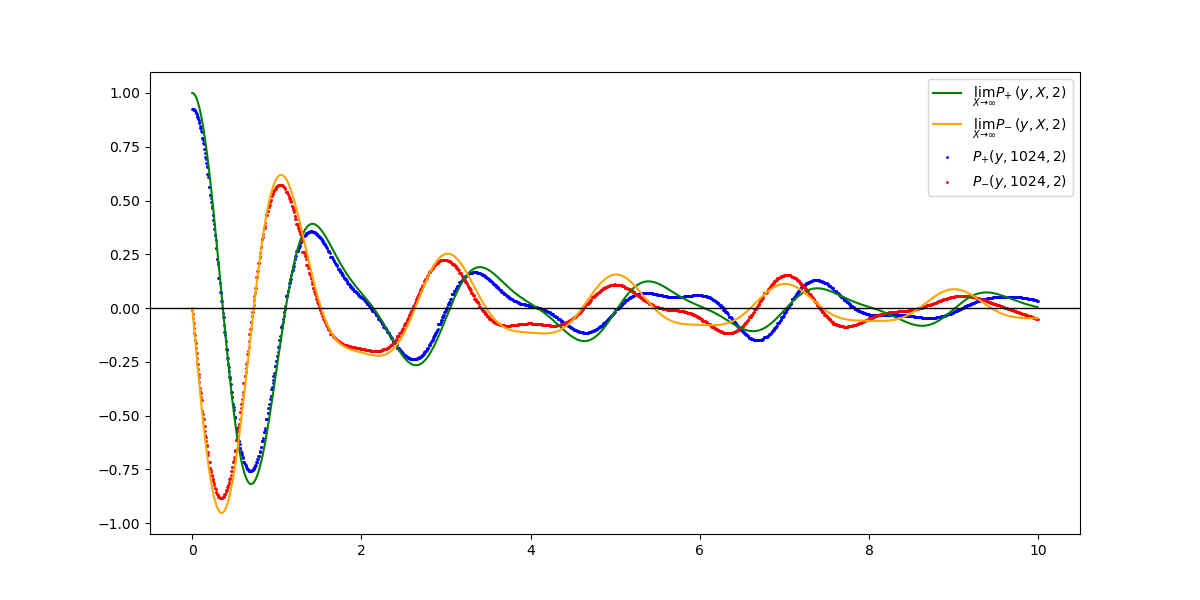
\includegraphics[width=\textwidth]{src/lop_fig1_top.png}%
        \label{fig:lop_fig1_top}
    \end{subfigure}
    
    \begin{subfigure}{1.0\textwidth}
        \centering
        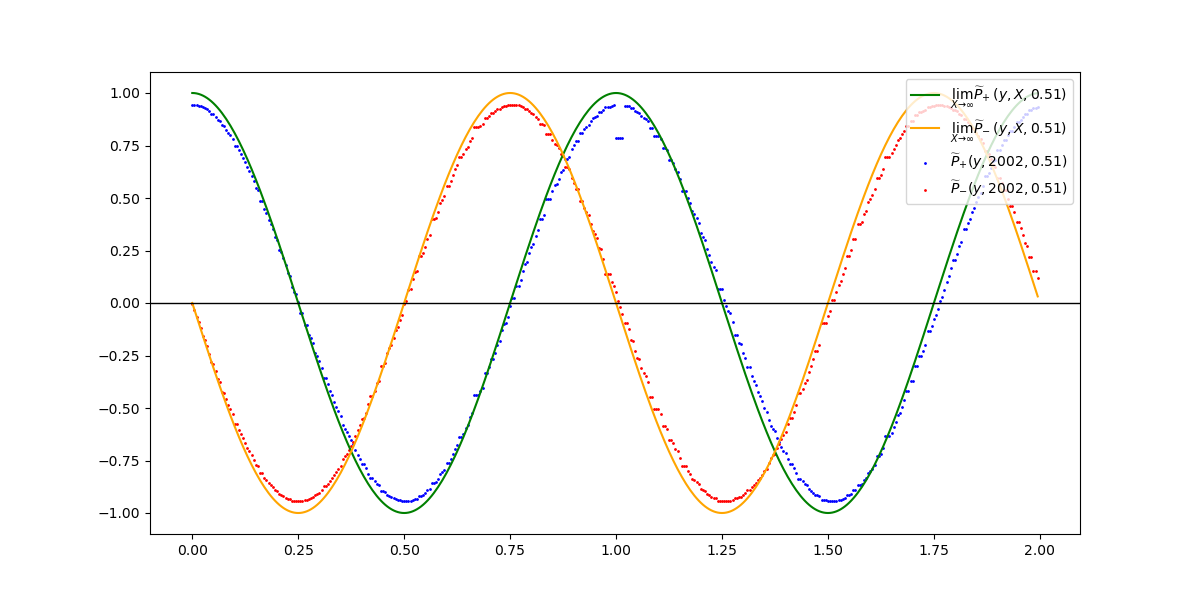
\includegraphics[width=\textwidth]{src/lop_fig1_bottom.png}%
        \label{fig:lop_fig1_bottom}
    \end{subfigure}

    \caption{Murmuration of Dirichlet characters. The top figure presents $P_{\pm}(y, 2^{10}, 2)$ for $y \in [0, 10]$ with $+$ in blue and (the imaginary part of) $-$ in red. The bottom figure presents $\widetilde{P}_{\pm}(y, 2002, 0.51)$ for $y \in [0, 2]$ with $+$ in blue and (the imaginary part of) $-$ in red. The discontinuity of $\widetilde{P}_{+}(y, 2002, 0.51)$ at $y = 1$ corresponds to the term $p = N$ in \eqref{eqn:lee_2_avg}.}
\label{fig:lop}
\end{figure}


\begin{figure}[htp] 
\centering
    \begin{subfigure}{1.0\textwidth}
        \centering
        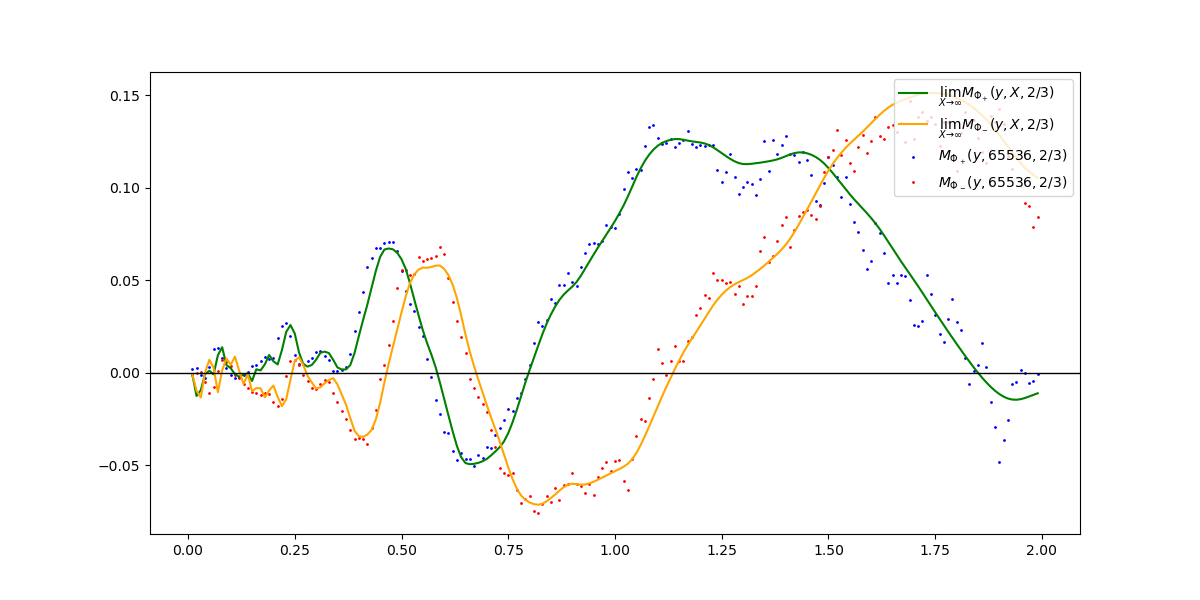
\includegraphics[width=\textwidth]{src/lop_fig2.png}%
        \label{fig:lop_fig2}
    \end{subfigure}
    
    \begin{subfigure}{1.0\textwidth}
        \centering
        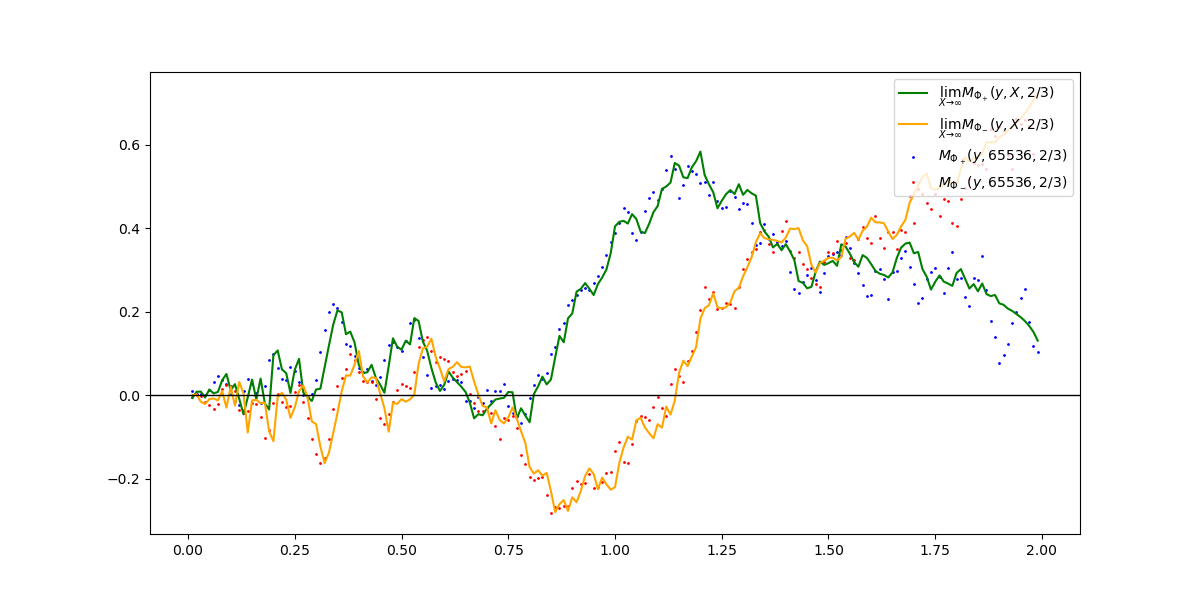
\includegraphics[width=\textwidth]{src/lop_fig3.png}%
        \label{fig:lop_fig3}
    \end{subfigure}

    \caption{Murmuration of Kronecker characters $\chi_{8d}$. The top figure presents $M_{\Phi_{\pm}}(y, 2^{16}, \frac{2}{3})$ for $y \in [0, 2]$ with $\Phi_+(x) = \1_{(1, 2)}(x) \exp(-1/(1 - 4(x - \frac{3}{2})^2))$ and $\Phi_-(x) = \1_{(-2, -1)}(x) \exp(-1/(1 - 4(x + \frac{3}{2})^2))$. The bottom figure presents $M_{\Phi_{\pm}}(y, 2^{16}, \frac{2}{3})$ for $y \in [0, 2]$ with $\Phi_+(x) = \1_{(1, 2)}(x)$ and $\Phi_-(x) = \1_{(-2, -1)}(x)$. Note that we use $\gamma = \frac{2}{3}$, even if the above proof only works when $\gamma > \frac{3}{4}$.}
\label{fig:lop_quad}
\end{figure}